\documentclass{article}
\usepackage[a4paper, margin=2cm]{geometry} 
\usepackage[T1]{fontenc} %lädt Deutsche schriftzeichen
\usepackage{amssymb}%für Mathe
\usepackage{setspace} %für Zeilen Abstand 
\usepackage[none]{hyphenat} % Silbentrennung deaktivieren 
\usepackage{fancyhdr}%Kopf und Fußzeile: https://de.overleaf.com/learn/latex/Headers_and_footers
\usepackage{graphicx}%Zum Bilder einfügen
\usepackage{xcolor}
\usepackage{wrapfig}
%\usepackage[document]{ragged2e}%für Blocksatz
\usepackage[ddmmyyyy]{datetime}%zum bearbeiten vom Datungs Format
\usepackage{eurosym}%für \Euro / \euro
\usepackage{hyperref}


\newcommand{\authoren}{Niklas Hainz}
\newcommand{\Thema}{Spiel Projekt}
\newcommand{\Fach}{Praktische Informatik}
\newcommand{\Zeilenabstand}{1.2}
\newcommand{\Inhaltsverzeichnisname}{Inhaltsverzeichnis}


\newcommand{\absatz}{5mm}
\newcommand{\Blocksatz}{\justifying}
\newcommand{\strich}{\vspace{\absatz}\hrule\vspace{\absatz}} 


\title{\Thema}
\author{\authoren}
\date{\today}


\setlength{\parindent}{0cm} %deaktiviert die Automatische Einrückung am Anfang des Dokumentes 
\renewcommand{\contentsname}{\Inhaltsverzeichnisname}
\renewcommand{\dateseparator}{.}







\begin{document}
\begin{spacing}{\Zeilenabstand}
\maketitle
\begin{center}
    \vspace{-\absatz}
    \Fach
\end{center}
\thispagestyle{empty}
\newpage

\pagestyle{fancy}
\fancyhead[L]{\authoren}
\fancyhead[C]{\Thema / \Fach}
\fancyhead[R]{\today}
\fancyfoot[R]{\thepage}
\fancyfoot[C]{}

\pagenumbering{roman}
\setcounter{page}{1}
\tableofcontents


\newpage

\pagenumbering{arabic}
\setcounter{page}{1}


%%% Document start %%%



%\section{Einleitung}

\section{Planung}

\subsection{Produktskizze}

Das geplante Spiel soll den gleichen Aufbau und Ablauf wie das Spiel "Bubble Bobble" haben: Das Spiel besteht aus mehreren Leveln, welche alle eine Verschiedene Anzahl und Typen an Gegnern beinhalten. Diese Gegnere müssen alle Besigt werden um in das nächste Level zu kommen. Die Gegner sind besiegbar mit Blasen die vom Spieler aus geschoßen werden können.


\subsubsection{Ziel des Spieles}

Das Ziel des Spieles ist es alle Level zu bestehen.


\subsubsection{Genre des Spiels}

Das Spiel ist das Genre Jump `n' Run 

\subsubsection{Grobe Struktur der Benutzeroberfläche}

Oben in der Mitte soll immer der Highscore und der Score vom ersten Spieler links und den Score von dem Zweiten Spieler unten Links sollte noch die Leben in form von Blasen angezeigt werden.

\subsubsection{Aufgaben und Vorgehen des Spielers}

Der Spiel muss alle Gegner besiegen bis er ins nächste Level kommt. 

\subsubsection{Spielende}

Das Spielende tritt ein wenn Spieler eins und Spieler zwei keine Leben mehr haben, dann wird ein ``Game over'' screen eingeblendet.

\subsection{Prototypen}

\begin{figure}[h]
    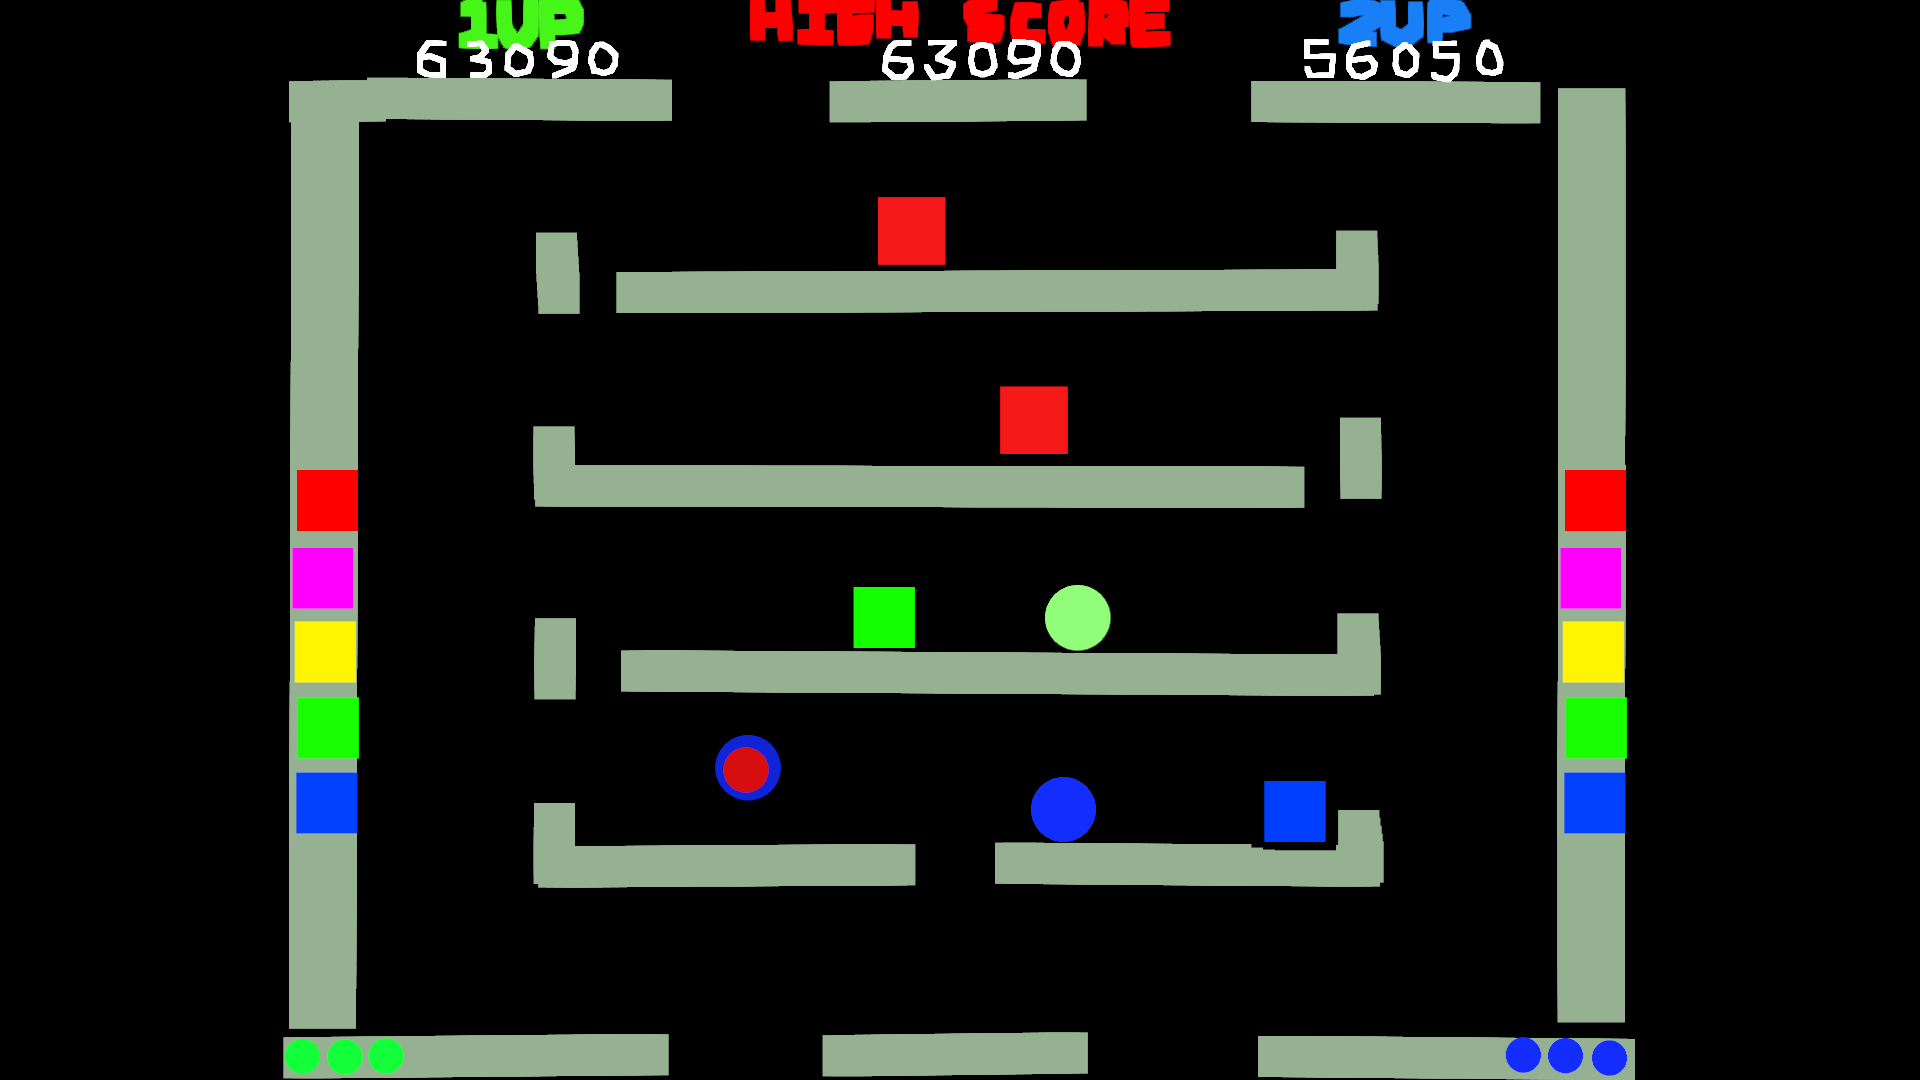
\includegraphics[scale=0.5]{media/Bubble_bobble_remake_proto.png}
    \label{Bubble_Bobble_remake_Proto}
\end{figure}

Die Roten Rechtecke in der Mitte sind gegner. Das blaue und das Grüne Rechtecke sind Spieler eins(Grün) Spieler zwei(Blau).Die Rechtecke links und Rechts sind für ein Bonus Leben. Oben in der Mitte ist der Highscore der, der gleiche ist wie der höchste Spieler punktzahl oder wenn der einer der Aktuellen spielern ein Höhren Highscore hat dann wird dieser ersetzt und Geupdate.


\subsubsection{Spielbeginn}

Zu Spiel beginn muss entweder eine virtuelle Münze eingeworfen werden(Start Taste) oder das Spiel Starte direkt 

\subsubsection{Typische Szene im Spiel}

Spieler kämpt gegen Gegner um ins Nächste Level zu kommen. Ggf. Zwei Spieler.

\subsubsection{Spielende}

Spiel ende Trifft eine wenn beide Spieler keine Leben mehr haben. Dann würde der  ``Game Over''  Screen eintreten 

\subsection{Versionierung}

Versionierung mit Git.
Plannung sind mindesten 20 Level wünschenswert währen mehr bis alle 100 und einführung von den Bonbons als Powerups auch hier wäres wünschens wert wenn es noch mehr Items hinzugefügt werden.
Selbst erstelle Sprites. 

%\section{Entwurf}
%
%\subsection{Struktogramm(e) einer (von)  Methode(n)}
%
%\section{Durchführung}
%
%\subsection{Beschreibung Ablauf }
%
%\subsection{Beschreibung des Spielablaufs}
%
%\subsection{Fehlerprotokoll und Maßnahmen zur Behebung}
%
%\subsection{Kommentierter Quelltex}
%
%\subsection{Begründung von Abweichungen gegenüber Planung}
%
%\subsection{Screenshots}
%
%\section{Fazit}
%
%\section{Quellen}

\end{spacing}
\end{document}